\section{Introduction}
\label{sec:intro}
Deep neural models have shown to be effective in 
a large variety of natural language inference~(NLI)
tasks~\cite{bowman2015large,wang2018glue,mostafazadeh2016corpus,roemmele2011choice,zellers2018swag}. Many of these tasks
are discriminative by nature, such as predicting a class label or
an outcome given a textual context, as shown in the following example:

\begin{example}\label{exp:snli}
Natural language inference in SNLI dataset, with ground truth bolded.
\begin{description}
\item{Premise:} A swimmer playing in the surf watches a low flying airplane headed inland. 
\item{Hypothesis:} Someone is swimming in the sea.
\item{Label:} \textbf{a) Entailment.} b) Contradiction.  c) Neutral.
\end{description}
\end{example}

The number of candidate labels may vary. Humans solve such questions by
reasoning the logical connections between the premise and the hypothesis,
but previous work~\cite{naik2018stress,schuster2019towards} 
has found that some NLP models can solve the questions
fairly well by looking only at the hypothesis (or ``conclusion'' in some work)
in the datasets.
It is widely speculated that this is because in many datasets, 
the hypotheses are manually crafted and may contain artifacts that
would be predictive of the correct answer. 
Such ``hypothesis-only'' tests can identify problematic questions
in the dataset if the question can be answered correctly without 
the premise. While such a method to evaluate the quality of
a dataset is theoretically sound, 
it i) usually relies on training a heavy-weight model such as BERT, which
is costly to evaluate, ii) does not provide explanation why the question is 
a culprit, and iii) cannot be used to evaluate a model since a model that
can make a correct prediction using only the hypothesis is not necessarily a
bad model: it is just not given the complete data.  


%argumentation~\cite{niven2019probing}, commonsense reasoning~\cite{}, 
%reading comprehension~\cite{lai2017race}, question answering~\cite{talmor2019commonsenseqa} 
%and dialogue analysis~\cite{lowe2015ubuntu}. 

Inspired by black-box testings in software engineering, 
CheckList~\cite{checklist2020acl} assesses the weakness of 
models without the need to know the details of the model. It does so by
providing additional stress test cases according to predefined 
linguistic features. Unfortunately, to ensure the correctness of
these additional cases, the templates must be carefully crafted
with substantial restrictions, thus limiting the testing space and
complicating the implementation. 
Furthermore, with CheckList, you only get to know what the model 
is incapable of doing but won't know what the model has 
learned from the data.

%\begin{figure}[th]
%\centering
%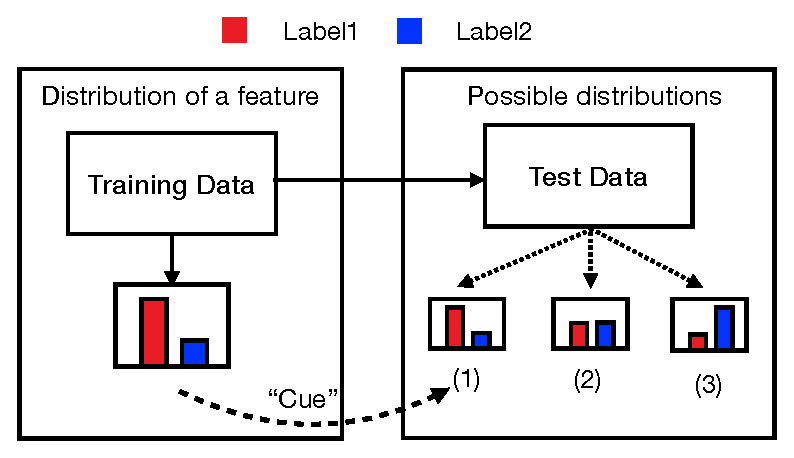
\includegraphics[width=0.6\columnwidth]{picture/cue_def.eps}
%\caption{Example of a {\em cue}. }
%%\KZ{``Possible distributions of the same feature''}}
%\label{fig:cue_def}
%\end{figure}

In this paper, our view is that the existing test sets for these
tasks are not sufficiently exploited. Why do we go the extra mile to
generate new test cases which are potentially incorrect, when we can
test the models using existing test sets but from different perspectives?
With this objective in mind, we propose an algorithm to statistically 
determine possible biases that exist in a dataset.
%evaluating both the dataset and the corresponding models. In this framework, 
%one test dataset can be seen as multiple test sets from different perspectives. 
%which
%In this paper, we propose a light-weight framework called
%can evaluate both the {\em data set} and the {\em model} for
%discriminative NLI tasks {\em fully} automatically. 

Previous studies~\cite{gururangan2018annotation,sanchez2018behavior,poliak2018hypothesis} 
showed that statistical bias on linguistic features 
(e.g., sentiment, repetitive words and even shallow n-grams)
which have statistical correlation with specific labels 
in benchmark datasets can be predictive of the correct 
answer. We call such features artificial spurious \textit{cues} when
the correlation is particularly strong.
%We illustrate this in~\figref{fig:cue_def}. 
%Once these cues are neutralized from the test data, 
%previously successful models may degrade substantially
%on it, suggesting that the model has taken advantage of 
%the biased feature and is hence not as robust as assumed 
%against with such cues.

%Inspired by the black-box testing in CheckList, 
%%whwith various of perturbation strategies, like typos, 
%we propose to generate test cases by just 
%filtering the original test data into new subsets according to 
%specific linquistic features, like word, NER, Negation, and sentiment, etc. 
%%in constructing the spurious cues. 
%We can show the cases distribution on each label indicates whether 
%the dataset is balance on this feature. In another word, we can 
%find the bias and cues intuitively. 
%Meanwhile,  we can prob what bias features the model really sensitive to.
%We even out the filtered test date on different labels. The even out version 
%can be used as a ``feature test'' to estimate whether a model consider 
%bias features in training data to make prediction.
%
%Our framework can be used to identify simple but effective biases and cues  
%in a broad range of multiple choice NL reasoning datasets.
%Though not all multiple choice questions in these dataset involve 
%all three components, i.e., a premise, a hypothesis and a label, 
%we will describe in~\secref{sec:formulation} how to normalize them into
%the standard form. 

%The relative size of hard part over the whole
%data indicates the quality of the dataset .
%\KZ{pls quickly finish the remaining part of intro. 
%The contributions part is critical.}
%Thus we can
%separate the original dataset into easy and hard part with 
%the bias score feature of cues
%any   dataset into easy and hard part
%and thus we can evaluate the ``biasness'' and ``quality'' of the dataset. 



%using simple and cost-effective linear classification models 
%on the simple cue features,
%which trained with unbalanced score of cues to several benchmark datasets across 
%various tasks and domains. 
%We evaluate the effectiveness of our methods with the 
%deviation between our results and random selection results. 
%Simultaneously, the test set can be divided into two parts: \textbf{easy} and \textbf{hard}. 
 %\textbf{balance} and \textbf{imbalance} are relative rather than absolute. 
%\KZ{Improving the neural models by splitting the training set.} 

%The training data can be separated into $n$ parts, test on one part and training 
%the model on the rest for each time. 
%The filtered part contains the instances 
%which can not be correctly chosen.
%The filtered data will be used to train a better model for target tasks. 

In summary, this paper makes the following contributions:
%\KZ{These contribs need to be revised right?}
\begin{itemize}
\item we provide a light-weight but effective model-independent method to 
uncover the statistical cues in NL reasoning datasets;
%(\secref{sec:result}).

\item we propose a simple blackbox test to quantitatively 
assess whether a given model has taken advantage of a
spurious cue when making predictions;

\item we evaluate the statisical bias issues comprehensively on
10 popular NLR datasets and 4 models and confirmed that many of the
top cues we discovered are indeeded exploited by the models.
%\item we created an online demonstration system to showcase
%the results and invite users to evaluate their own datasets and models.
\end{itemize}
% (\secref{sec:result}).

%\item We filter the training data and get a better performance on the \textbf{hard} dataset.
%to get a high quality training dataset which
 %is possibly closer to the intended task. 







